\documentclass[11pt]{amsart}
\pdfsuppressptexinfo=-1
\usepackage[margin=1.1in]{geometry}
\usepackage{amsmath,amssymb,amsthm,mathtools}
\usepackage{booktabs,enumitem,array}
\usepackage{tikz}
\usepackage[hidelinks]{hyperref}

\newtheorem{theorem}{Theorem}[section]
\newtheorem{lemma}[theorem]{Lemma}
\newtheorem{proposition}[theorem]{Proposition}
\newtheorem{corollary}[theorem]{Corollary}
\theoremstyle{definition}
\newtheorem{definition}[theorem]{Definition}
\theoremstyle{remark}
\newtheorem{remark}[theorem]{Remark}
\numberwithin{equation}{section}
\setlength{\emergencystretch}{2em}
\raggedbottom

\newcommand{\DB}{\mathrm{DB}}
\newcommand{\file}[1]{\texttt{#1}}
  \newcommand{\cc}{\frac43}\newcommand{\ccs}{4/3}\newcommand{\ccdec}{1.3333\ldots}
  \newcommand{\ttitle}{A thrackle on $n$ vertices has fewer than $4n/3$ edges}
  \newcommand{\ptitle}{A thrackle on n vertices has fewer than 4n/3 edges}
  \newcommand{\rtitle}{Thrackles have fewer than $4n/3$ edges}
\hypersetup{pdftitle={\ptitle},pdfauthor={Tejasvi Singh Tomar}}
\newcommand{\NSTATESALL}{1{,}215{,}372}
\newcommand{\NSTATES}{694{,}211}
\newcommand{\NTESTS}{207{,}380{,}593{,}775}
\newcommand{\WALLSUM}{7{,}765{,}559}
\newcommand{\NSTATESB}{26{,}550}
\newcommand{\NTESTSB}{3{,}520{,}550{,}932}
\newcommand{\WALLSUMB}{128{,}254}
\newcommand{\NTESTSC}{6{,}024{,}873}
\newcommand{\NCEIGHT}{2{,}544}
\newcommand{\NHONE}{60{,}196}
\newcommand{\NCLASSES}{343}
\newcommand{\NSTATESD}{1{,}211{,}878}
\newcommand{\NSTATESDNINE}{32{,}626}
\newcommand{\NTESTSD}{83{,}401{,}645{,}992}
\newcommand{\WALLSUMD}{2{,}439{,}459}
\newcommand{\NCTEN}{6{,}059{,}712}
\newcommand{\NCNINE}{72{,}916}
\newcommand{\SUPPDOI}{10.5281/zenodo.23716511}
\newcommand{\REPOURL}{https://github.com/tejasvi/thrackle-bound/tree/v4}

\begin{document}

\title[\rtitle]{\ttitle}
\author{Tejasvi Singh Tomar}
\renewcommand{\urladdrname}{{\itshape ORCID}}
\urladdr{\href{https://orcid.org/0000-0003-4668-3639}{https://orcid.org/0000-0003-4668-3639}}
\subjclass[2020]{05C10, 05C35; 05C62, 68R10}
\keywords{Thrackle, Conway's thrackle conjecture, topological graph, discharging, planarity testing, computer-assisted proof, formal verification}

\begin{abstract}
A thrackle is a drawing of a graph in the plane in which every two edges meet exactly once, either at a common endpoint or at a proper crossing. Conway conjectured that a thrackle with $n$ vertices has at most $n$ edges. We prove that a thrackle with $n\ge4$ vertices has at most $\cc(n-1)$ edges, improving the bound $\frac{18}{13}(n-1)$ obtained by T\'oth and, independently, by Scoppetto. The proof combines Xu's discharging argument with two computer searches, by the method of Fulek and Pach, showing that two dumbbells are not thrackleable: a $6$-cycle and an $8$-cycle sharing one edge, and a $6$-cycle and a $10$-cycle sharing a path of three edges. A formal proof in Lean~4 derives the bound from five properties of thrackles and checks the computational facts it uses; Section~\ref{sec:lean} states what this proof trusts.
\end{abstract}

\maketitle

\section{Introduction}\label{sec:intro}

A \emph{drawing} of a graph in the plane represents the vertices by distinct points and the edges by simple arcs between the points of their endpoints, so that no arc passes through a vertex other than its endpoints, two arcs have finitely many common points, and two arcs never touch without crossing. A \emph{thrackle} is a drawing in which every two edges meet exactly once: two edges with a common endpoint meet only there, and two edges without a common endpoint cross exactly once, properly. A graph is \emph{thrackleable} if it has a thrackle drawing. Let $t(n)$ be the largest number of edges of a thrackleable graph with $n$ vertices. Conway's thrackle conjecture states that $t(n)\le n$ for every $n$. It would be sharp, since every cycle of length at least five is thrackleable \cite{Woo71}, \cite[Section~1]{FP11}.

Lov\'asz, Pach and Szegedy proved $t(n)\le2n-3$ for $n\ge2$ \cite{LPS97}, and the constant was lowered several times since \cite{CN00,FP11,GX17,FP19,Xu21}. Fulek and Pach introduced a computational method for deciding whether a small graph is thrackleable \cite{FP11}, and Xu's discharging argument gives $t(n)\le1.393(n-1)$ for $n\ge4$ \cite{Xu21}, \cite[Section~3.1]{Sco26}. The constant $\frac{18}{13}$ appeared in \cite[Remark~2]{FP19}, conditional on a computer verification of the conjecture for $n\le11$ that had been stated without proof in \cite{CN09}. In 2026 the bound $\frac{18}{13}(n-1)$ was obtained by T\'oth in a bachelor thesis \cite{Tot26} and, independently and for $n\ge4$, by Scoppetto \cite[Theorem~1.1]{Sco26}. Scoppetto shows with an adapted reconstruction of the program of Fulek and Pach that the dumbbell $\DB(6,8,-2)$ is not thrackleable, deduces that every $8$-face of the embedding used by Xu (Lemma~\ref{lem:embed}) has at most four edges in common with $6$-faces, and adapts Xu's discharging. We prove the following.

\begin{theorem}\label{thm:main}
Every thrackleable graph with $n\ge4$ vertices has at most $\cc(n-1)$ edges.
\end{theorem}

Since $t(1)=0$, $t(2)=1$ and $t(3)=3$, Theorem~\ref{thm:main} gives $t(n)<\cc n$ for every $n\ge1$.

For integers $c',c''\ge3$ and $0<k<\min(c',c'')$, the dumbbell $\DB(c',c'',-k)$ is the union of a $c'$-cycle and a $c''$-cycle whose intersection is a path with $k$ edges, and $\DB(c',c'',0)$ is the union of a $c'$-cycle and a $c''$-cycle with exactly one common vertex \cite{FP11}. The dumbbell $\DB(c',c'',-k)$ has $c'+c''-k-1$ vertices and one more edge than vertices, so a thrackleable dumbbell would disprove Conway's conjecture. Scoppetto pointed out \cite[Section~7.2]{Sco26} that if $\DB(6,8,-1)$ is not thrackleable, and if this forces every $8$-face to have no edge in common with a $6$-face, then the discharging would give $\frac{15}{11}$. We carry this out, and we go further by bounding the number of edges that a face of size~$10$ has in common with $6$-faces. The new computational ingredients are the following.

\begin{theorem}\label{thm:db}
The dumbbells $\DB(6,8,-1)$ and $\DB(6,10,-3)$ are not thrackleable.
\end{theorem}

\begin{figure}[ht]
\centering
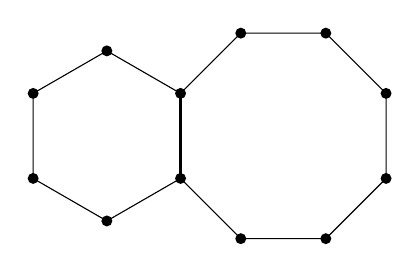
\begin{tikzpicture}[scale=0.9,every node/.style={circle,fill,inner sep=1.4pt}]
\coordinate (a) at (0,0.6); \coordinate (b) at (0,-0.6);
\foreach \i/\x/\y in {1/-1.04/1.2,2/-2.08/0.6,3/-2.08/-0.6,4/-1.04/-1.2} \coordinate (h\i) at (\x,\y);
\foreach \i/\x/\y in {1/0.85/1.45,2/2.05/1.45,3/2.9/0.6,4/2.9/-0.6,5/2.05/-1.45,6/0.85/-1.45} \coordinate (o\i) at (\x,\y);
\draw[very thick] (a)--(b);
\draw (a)--(h1)--(h2)--(h3)--(h4)--(b);
\draw (a)--(o1)--(o2)--(o3)--(o4)--(o5)--(o6)--(b);
\foreach \p in {a,b,h1,h2,h3,h4,o1,o2,o3,o4,o5,o6} \node at (\p) {};
\end{tikzpicture}
\caption{The dumbbell $\DB(6,8,-1)$: a $6$-cycle and an $8$-cycle sharing one edge (thick). It has $12$ vertices and $13$ edges.}\label{fig:db}
\end{figure}

We prove Theorem~\ref{thm:db} with the method of Fulek and Pach \cite{FP11}: a graph $G$ is thrackleable if and only if, for some choice of the orders in which the edges cross each other, an associated graph $G'$ is planar. Our search builds these orders edge by edge, tests the planarity of the partial graphs, and prunes with the complete lists of admissible orders for subgraphs, following an idea of Scoppetto \cite{Sco26}. Section~\ref{sec:search} describes the search and the computations.

Smaller computations, collected in Section~\ref{sec:comp}, show that in a triangle-free thrackleable graph no $6$-cycle shares an edge with an $8$-cycle and two distinct $6$-cycles have no common vertex, and that $\DB(5,5,-2)$ and $\DB(5,6,-2)$ are not thrackleable. The second of these facts is used in \cite{FP19,Sco26}, although only its dumbbell cases had been checked.

Section~\ref{sec:proof} then proves Theorem~\ref{thm:main} along the lines of Xu \cite{Xu21} and Scoppetto \cite{Sco26}. A $2$-connected triangle-free thrackleable graph has an embedding in the plane or the projective plane in which every face has even size, hence size at least six. In this embedding these facts show that the faces adjacent to a $6$-face have size at least $10$, and, with a further enumeration, that a face of size~$10$ has at most six edges in common with $6$-faces; a discharging argument then gives the bound for triangle-free graphs. Conway's doubling reduces graphs with a triangle to bipartite ones, and disconnected graphs are handled separately. Section~\ref{sec:lean} describes a proof of Theorem~\ref{thm:main} in Lean that also checks all the computational facts, including the two large searches. Section~\ref{sec:remarks} explains why these facts give exactly the constant $\cc$.

\section{Preliminaries}\label{sec:prelim}

All graphs are finite and simple. For a graph $G$ we write $n$ for the number of vertices and $m$ for the number of edges, and $C_k$ for the cycle of length $k$. A subgraph of a thrackleable graph is thrackleable, since deleting edges and vertices from a thrackle leaves a thrackle. We use the following known facts.

\begin{lemma}[{\cite[Lemma~4]{FP19}}]\label{lem:c4}
The cycle $C_4$ is not thrackleable.
\end{lemma}

In fact, $C_4$ cannot even be drawn so that every two edges without a common endpoint cross an odd number of times and adjacent edges meet only at their common endpoint \cite[Lemma~4 and Section~5]{FP19}.

Let $G$ be drawn as a thrackle, and let $C$ be an odd cycle of $G$. Conway's doubling of $C$ replaces every vertex $v$ of $C$ by two nearby vertices $v_1,v_2$, every edge $vv'$ of $C$ by the two edges $v_1v_2'$ and $v_2v_1'$, and attaches each other edge at $v$ to $v_1$ or to $v_2$, according to the side of $C$ on which it leaves $v$, so that every edge attached to $v_1$ crosses every edge attached to $v_2$ exactly once near $v$; all other edges are kept \cite[Section~2]{FP11}. The cycle $C$ of length $k$ becomes a cycle of length $2k$, so the number of vertices and the number of edges both grow by $k$.

\begin{lemma}[Conway; {\cite[Lemma~5]{FP11}}; see also {\cite[Lemma~2]{CN00}}]\label{lem:double}
Let $G$ be drawn as a thrackle, and let $C$ be an odd cycle of $G$. Then the graph obtained by Conway's doubling of $C$ is bipartite, and it can be drawn as a thrackle.
\end{lemma}

An embedding of a graph in the projective plane is a \emph{parity embedding} if every odd cycle is one-sided and every even cycle is two-sided. In a parity embedding every face has even size, where the size of a face is the length of its facial walk \cite[Section~2]{FP19}.

\begin{lemma}[{\cite[Corollary~1 and Proposition~1]{FP19}}, based on \cite{LPS97,CN09}]\label{lem:embed}
Let $G$ be a $2$-connected triangle-free thrackleable graph. If $G$ is bipartite, it has an embedding in the plane; otherwise it has a parity embedding in the projective plane. In either embedding every face has even size, and the facial walk of every face of size at most $8$ is a cycle.
\end{lemma}

Both embeddings are cellular: in the plane since $G$ is connected, and in the projective plane since $G$ contains an odd cycle $C$, which is one-sided, so that the complement of $C$ is an open disc, and the faces of the connected graph $G\supseteq C$ in this disc are open discs. So every face has one facial walk, and every edge is traversed twice by the facial walks, once on each side. In the plane case the last statement of Lemma~\ref{lem:embed} holds for all faces, by the $2$-connectivity of $G$.

Proposition~1 of \cite{FP19} is stated for $2$-connected thrackles, but its proof (in the arXiv version of \cite{FP19}) uses that $G$ is triangle-free; since that proof is brief, we include one for the projective case. There every odd cycle is one-sided and every even cycle two-sided, so a closed walk has odd length if and only if it is one-sided, that is, nonzero in the homology of the projective plane with coefficients in $\mathbb Z_2$ (decompose its edges, counted modulo~$2$, into cycles). Let $W$ be the facial walk of a face $D$ of size at most $8$. Suppose first that $W$ traverses an edge $e$ twice. A simple closed curve $\gamma$ that runs through $D$ and meets $G$ only once, crossing $e$, does not separate the projective plane, because $e$ is not a bridge of $G$; so $\gamma$ is one-sided, and $W=ePeQ$ traverses $e$ twice in the same direction. The closed walks $eP$ and $eQ$ cross $\gamma$ once, so they have odd length, which is at least $3$ since $G$ has no loops; as their lengths add up to $|W|\le8$, one of them has length $3$ and is a triangle. If $W$ traverses no edge twice but repeats a vertex, it splits into two closed trails of total length at most $8$, one of which has length $3$ or $4$ and is a triangle or a $4$-cycle. Both cases are excluded, so $W$ is a cycle.

For an edge $e$ of a graph $G$, let $N(e)$ be the set of edges of $G$ that have no endpoint in common with $e$. Orient every edge of $G$. A \emph{crossing system} $\Pi=(\pi_e)_{e\in E(G)}$ consists of a linear order $\pi_e$ of $N(e)$ for every edge $e$; in a thrackle, $\pi_e$ is the order in which the edges of $N(e)$ cross $e$ when $e$ is traversed in its direction. Given $\Pi$, the \emph{augmented graph} $G'(G,\Pi)$ is obtained as follows \cite[Section~4]{FP11}. Each edge $e$ becomes a path from its tail to its head through one new vertex $X_{ef}$ for each $f\in N(e)$, in the order $\pi_e$, with one further new vertex between any two consecutive crossing vertices; the vertex $X_{ef}=X_{fe}$ lies on the paths of both $e$ and $f$. Finally, for every crossing vertex $X=X_{ef}$, with neighbours $a_1,a_2$ on the path of $e$ and $b_1,b_2$ on the path of $f$, the $4$-cycle $a_1b_1a_2b_2$ is added.

\begin{lemma}[{\cite[Section~4]{FP11}}]\label{lem:fp}
A graph $G$ is thrackleable if and only if $G'(G,\Pi)$ is planar for some crossing system $\Pi$.
\end{lemma}

\begin{proof}[Sketch]
A thrackle gives $\Pi$ and a plane drawing of $G'(G,\Pi)$: the crossings become vertices, and the $4$-cycles can be drawn along the arcs, close to the crossings. Conversely, in an embedding of $G'(G,\Pi)$ in the plane the $4$-cycle around $X_{ef}$ together with the four edges at $X_{ef}$ form a wheel, which is $3$-connected and therefore has a unique embedding up to reflection; so the two edges of the path of $e$ at $X_{ef}$ are separated by those of $f$. Deleting the $4$-cycles and turning the vertices $X_{ef}$ into crossings gives a drawing in which every two edges without a common endpoint cross exactly once, at a proper crossing, and adjacent edges meet only at their common endpoint.
\end{proof}

\section{The computational results}\label{sec:comp}

Besides Theorem~\ref{thm:db}, the proof of Theorem~\ref{thm:main} uses the following computational facts.

\begin{theorem}\label{thm:dbs}
The dumbbells $\DB(6,8,-2)$ and $\DB(6,8,-3)$ are not thrackleable.
\end{theorem}

For $\DB(6,8,-2)$ this is \cite[Lemma~4.2]{Sco26}. For $\DB(6,8,-3)$, which is also $\DB(8,8,-5)$ and has $10$ vertices, \cite[Lemma~3.13]{Sco26} relies on the statement in \cite{FP11} that Conway's conjecture holds for bipartite graphs with at most $10$ vertices; since the computations in \cite[Section~4]{FP11} concern the dumbbells $\DB(6,6,\ell)$, we checked $\DB(6,8,-3)$ directly. The proof of Theorem~\ref{thm:dbs} is the computation described in Section~\ref{sec:search}.

\begin{lemma}\label{lem:overlap}
Let $C$ be a $6$-cycle and $F$ an $8$-cycle of a triangle-free thrackleable graph, and suppose that $C$ and $F$ have at least one common edge. Then $C\cup F$ is $\DB(6,8,-1)$.
\end{lemma}

\begin{proof}
Write $F=v_0v_1\dots v_7$ and $C=w_0w_1\dots w_5$, where $w_0w_1=v_0v_1$ is a common edge; after reflecting $F$ we may assume $w_0=v_0$ and $w_1=v_1$. Each of $w_2,\dots,w_5$ is either a vertex outside $F$ or one of $v_2,\dots,v_7$, distinct ones for distinct $w_i$. We enumerated all these choices by computer and sorted the graphs $C\cup F$ into isomorphism classes. There are $\NCLASSES$ classes. Of these, $266$ contain a triangle; of the others, $60$ contain a $4$-cycle; of the remaining $17$, four contain two distinct $6$-cycles with a common vertex (among them $\DB(6,8,-4)$, which is also $\DB(6,6,-2)$), three are the dumbbells $\DB(6,8,-k)$ for $k=1,2,3$, and $10$ are of none of these kinds. Graphs with a triangle are excluded by assumption, and graphs with a $4$-cycle are excluded by Lemma~\ref{lem:c4}. The dumbbells $\DB(6,8,-2)$ and $\DB(6,8,-3)$ are not thrackleable by Theorem~\ref{thm:dbs}. For the $4+10$ remaining classes the search of Section~\ref{sec:search} found no planar augmented graph, so they are not thrackleable. Hence $C\cup F=\DB(6,8,-1)$.
\end{proof}

\begin{corollary}\label{cor:noshare}
In a triangle-free thrackleable graph, no $6$-cycle has an edge in common with an $8$-cycle.
\end{corollary}

\begin{proof}
By Lemma~\ref{lem:overlap} the union of such cycles would be $\DB(6,8,-1)$, a subgraph of a thrackleable graph, contradicting Theorem~\ref{thm:db}.
\end{proof}

Fulek and Pach \cite[Section~3]{FP19} state that two distinct $6$-cycles of a thrackle have no common vertex, citing \cite{FP11}, where Lemma~6 shows that the dumbbells $\DB(6,6,-k)$, $0\le k\le3$, are not thrackleable (the case $k=3$ is due to Lov\'asz, Pach and Szegedy \cite[Theorem~5.1]{LPS97}). Since two $6$-cycles can also meet in more than one path or vertex, we checked these cases as in Lemma~\ref{lem:overlap}.

\begin{lemma}[see {\cite[Section~3]{FP19}}]\label{lem:six}
Two distinct $6$-cycles of a triangle-free thrackleable graph have no common vertex.
\end{lemma}

\begin{proof}
Let $Q=v_0\dots v_5$ and $Q'=w_0\dots w_5$ be distinct $6$-cycles with the common vertex $w_0=v_0$. Each of $w_1,\dots,w_5$ is a vertex outside $Q$ or one of $v_1,\dots,v_5$, distinct ones for distinct $w_i$. Up to isomorphism these choices give $84$ graphs $Q\cup Q'$. Of these, $56$ contain a triangle; of the others, $20$ contain a $4$-cycle; of the remaining eight, four are the dumbbells $\DB(6,6,-k)$ for $0\le k\le3$, and four are of none of these kinds.\ The dumbbells are not thrackleable by \cite[Lemma~6]{FP11} and \cite[Theorem~5.1]{LPS97}, and our program confirms this. For the remaining four\ graphs our program finds no planar augmented graph. With Lemma~\ref{lem:c4} this proves the claim.
\end{proof}

For the faces of size~$10$ we need, besides $\DB(6,10,-3)$, two further dumbbells. The dumbbells $\DB(5,5,-2)$, $\DB(5,6,-2)$ and $\DB(6,10,-3)$ are the graphs formed by three internally disjoint paths between two vertices, of lengths $2,3,3$, of lengths $2,3,4$ and of lengths $3,3,7$.

\begin{theorem}\label{thm:dbten}
The dumbbells $\DB(5,5,-2)$ and $\DB(5,6,-2)$ are not thrackleable.
\end{theorem}

The proof is again the computation of Section~\ref{sec:search}.

\section{Proof of Theorem~\ref{thm:main}}\label{sec:proof}

Throughout this section $c=\frac43$ and $r=2c=\frac83$.\ Lemma~\ref{lem:twoconn} uses the charges of \cite[proof of Theorem~1.1, Case~1]{Sco26}, which follow Xu \cite{Xu21}, and Lemmas~\ref{lem:trianglefree} and~\ref{lem:triangle} and the proof of Theorem~\ref{thm:main} follow Cases~1, 2 and~3 of the same proof. Let $G$ be a $2$-connected triangle-free thrackleable graph, embedded as in Lemma~\ref{lem:embed}. A \emph{$k$-face} is a face of size $k$. Every face has even size. A face of size $2$ or $4$ would have a cycle of length $2$ or $4$ as its facial walk, which is impossible since $G$ is simple and $C_4$ is not thrackleable (Lemma~\ref{lem:c4}). So every face has size at least $6$, and the facial walks of the $6$-faces and $8$-faces are cycles. For a face $D$, a \emph{$6$-edge} of $D$ is a traversal of an edge by the facial walk of $D$ such that the other side of this edge belongs to a $6$-face. An edge with a $6$-face on one side is traversed only once by the facial walk of the face on its other side, so the $6$-edges of $D$ correspond to the edges that $D$ has in common with $6$-faces. We consider the traversals of a facial walk in their cyclic order, and call a maximal sequence of consecutive $6$-edges a \emph{run}.

\begin{lemma}\label{lem:faces}
Let $G\ne C_6$ be a $2$-connected triangle-free thrackleable graph, embedded as in Lemma~\ref{lem:embed}.
\begin{enumerate}[label=(\alph*)]
\item Distinct $6$-faces have distinct boundary cycles.
\item Every edge of a $6$-face $D$ has a face of size at least $10$ on its other side.
\end{enumerate}
\end{lemma}

\begin{proof}
(a) Suppose that distinct faces $D,D'$ have the same cycle $Q$ as facial walk. At every vertex $v$ of $Q$ both $D$ and $D'$ occupy an angle between the two edges of $Q$ at $v$. If $v$ had a third edge, at most one of the angles at $v$ would be bounded by these two edges. So every vertex of $Q$ has degree $2$, and $G=Q$; for a $6$-face this means $G=C_6$, which is excluded.

(b) The facial walk of $D$ is a cycle $Q$ and traverses each edge $e$ of $Q$ once, so the other side of $e$ belongs to a face $D'\ne D$. If $D'$ were a $6$-face, its boundary cycle would, by (a), be a $6$-cycle different from $Q$ sharing the edge $e$ with it, contradicting Lemma~\ref{lem:six}. If $D'$ were an $8$-face, its boundary would be an $8$-cycle with the edge $e$ in common with $Q$, contradicting Corollary~\ref{cor:noshare}. Since $D'$ has even size at least $6$, it has size at least $10$.
\end{proof}

\begin{lemma}\label{lem:ten}
Let $G\ne C_6$ be a $2$-connected triangle-free thrackleable graph, embedded as in Lemma~\ref{lem:embed}. Then every $10$-face has at most eight $6$-edges.
\end{lemma}

\begin{proof}
Let $D$ be a $10$-face, and consider the ten traversals of its facial walk in their cyclic order. Two consecutive traversals share a vertex, at which the walk passes from one to the next. If both are $6$-edges, with $6$-faces $D_1$ and $D_2$ on their other sides, then the boundary cycles of $D_1$ and $D_2$ have this vertex in common, so they coincide by Lemma~\ref{lem:six}, and $D_1=D_2$ by Lemma~\ref{lem:faces}(a). Hence the $6$-edges of a run all have the same $6$-face $D^*$ on their other side. An edge traversed twice by the facial walk of $D$ has $D$ on both sides and gives no $6$-edge. So the $6$-edges of such a run are traversals of distinct edges of the boundary cycle of $D^*$, and there are at most six of them. In particular not all ten traversals are $6$-edges. If the $6$-edges form $b\ge2$ runs, these are cyclically separated by at least $b$ other traversals, so there are at most $10-b\le8$ of them; if $b\le1$, there are at most six.
\end{proof}
\begin{lemma}\label{lem:runs}
Let $G\ne C_6$ be a $2$-connected triangle-free thrackleable graph, embedded as in Lemma~\ref{lem:embed}. Then every run of $6$-edges of a $10$-face has at most two $6$-edges, and every $10$-face has at most six $6$-edges.
\end{lemma}

\begin{proof}
Let $D$ be a $10$-face with facial walk $W$. By the proof of Lemma~\ref{lem:ten}, the $6$-edges of a run all have the same $6$-face on their other side; let $Q$ be its boundary cycle. They are traversals of distinct edges of $Q$, so there are $s\le6$ of them. A facial walk returns along the edge it has just traversed only at a vertex of degree~$1$; since $G$ is $2$-connected, $W$ never does, so the run traverses $s$ consecutive edges of $Q$ (all of $Q$ if $s=6$). The other side of each edge of $Q$ is the $6$-face, not $D$, so every traversal of an edge of $Q$ by $W$ is a $6$-edge. Hence $W$ traverses each edge of $Q$ at most once, and by maximality the edges of $W$ just before and just after the run are not edges of $Q$. Label $Q=0\,1\,2\,3\,4\,5$ and $W=w_0w_1\dots w_9$ so that $w_i=i$ for $0\le i\le s$ (with $w_6=0$ if $s=6$). We enumerated by computer all closed walks $W$ in which each of $w_{s+1},\dots,w_9$ is a vertex of $Q$, an earlier vertex of $W$ or a new vertex (new vertices numbered in order of first appearance), such that: $W$ never returns along the edge it has just traversed, also at $w_0$; $w_sw_{s+1}$ and $w_9w_0$ are not edges of $Q$; $W$ traverses every edge of $Q$ at most once and every other edge at most twice; and the union of $Q$ and the edges of $W$ has neither triangles nor $4$-cycles. With this labelling, there is no such walk for $s=6$. For $s=5$ there are three, and in each of them the union contains two distinct $6$-cycles with a common vertex, which Lemma~\ref{lem:six} excludes. For $s=4$ there are four, and in each of them the union contains a $6$-cycle and an $8$-cycle with a common edge, which Corollary~\ref{cor:noshare} excludes. For $s=3$ there are $19$. In five of them the union contains two distinct $6$-cycles with a common vertex, and in five others a $6$-cycle and an $8$-cycle with a common edge. The remaining nine unions fall into five isomorphism classes: one is $\DB(5,5,-2)$, two contain it, one contains $\DB(5,6,-2)$, and one is $\DB(6,10,-3)$. Explicitly, in four of the nine walks $W$ contains a path of length~$2$ from $3$ to $0$ whose middle vertex is not on $Q$, which forms $\DB(5,5,-2)$ with $Q$; in four others $W$ contains a path of length~$3$, with inner vertices not on $Q$, between two vertices at distance~$2$ on $Q$, which forms $\DB(5,6,-2)$ with $Q$; in the last, $W$ is the run followed by a path of length~$7$ from $3$ to $0$ through new vertices. By Theorems~\ref{thm:db} and~\ref{thm:dbten} none of the nine unions is thrackleable. So every run has at most two $6$-edges. If the $6$-edges of $D$ form $b$ runs, there are at most $2b$ of them and, as in the proof of Lemma~\ref{lem:ten}, at most $10-b$ when $b\ge2$; so there are at most six.
\end{proof}

\begin{lemma}\label{lem:twoconn}
Let $G$ be a $2$-connected triangle-free thrackleable graph other than $C_6$. Then $m\le c(n-1)$, and $m\le c(n-2)$ if $G$ is bipartite.
\end{lemma}

\begin{proof}
Embed $G$ as in Lemma~\ref{lem:embed}, and let $f$ be the number of faces. Put $k=2$ if $G$ is bipartite and $k=1$ otherwise. Since the embedding is cellular, $n-m+f=k$ by Euler's formula.

Give every vertex $v$ the charge $d(v)-r$, where $d(v)$ is its degree, and every face $D$ of size $|D|$ the charge $\frac{r-2}2|D|-r$, which is $\frac{|D|-8}{3}$. The sum of the vertex degrees and the sum of the face sizes are both $2m$, so the total charge is
\[
2m-rn+(r-2)m-rf=-r(n-m+f)=-kr.
\]
Now let every face of size at least $10$ send $\frac19$ across each of its $6$-edges. By Lemma~\ref{lem:faces}(b), every $6$-face receives $\frac19$ across each of its six edges and ends with charge $-\frac23+\frac69=0$. An $8$-face sends nothing and keeps $0$. A $10$-face sends at most $\frac69$, by Lemma~\ref{lem:runs}, and keeps at least $\frac23-\frac69=0$. A face of size $d\ge12$ sends at most $\frac d9$ and keeps at least $\frac{d-8}3-\frac d9=\frac{2d-24}9\ge0$.\ The total charge does not change, so
\[
2m-rn=\sum_v\bigl(d(v)-r\bigr)\le-kr,
\]
that is, $m\le\frac r2(n-k)=c(n-k)$.
\end{proof}

\begin{lemma}\label{lem:trianglefree}
Every triangle-free thrackleable graph with $n\ge1$ vertices has at most $c(n-1)$ edges.
\end{lemma}

\begin{proof}
We use induction on $n$. If $G$ is disconnected, apply the induction hypothesis to its components $G_1,\dots,G_j$: then $m\le c(n-j)\le c(n-1)$. If $G$ is connected and has a cut vertex, then $G$ is the union of two connected graphs $G_1,G_2$ with exactly one common vertex, both smaller than $G$, and $m=m_1+m_2\le c(n_1-1)+c(n_2-1)=c(n-1)$. The graphs with one or two vertices satisfy the bound. If $G$ is $2$-connected, the bound follows from Lemma~\ref{lem:twoconn}, or from $6\le5c$ if $G=C_6$.
\end{proof}

\begin{lemma}\label{lem:triangle}
Every connected thrackleable graph with $n\ge4$ vertices that contains a triangle has at most $\cc(n-1)$ edges.
\end{lemma}

\begin{proof}
Draw $G$ as a thrackle, and let $H$ be the graph obtained by Conway's doubling of a triangle. By Lemma~\ref{lem:double}, $H$ is bipartite and thrackleable, and it is connected since $G$ is connected. It has $N=n+3\ge7$ vertices and $M=m+3$ edges, so $H\ne C_6$, and it contains the $6$-cycle that replaces the triangle. For a block $B$ of $H$ with $v_B$ vertices and $e_B$ edges, put $g(B)=c(v_B-1)-e_B$. Since $H$ is connected, $\sum_B(v_B-1)=N-1$, so
\[
c(N-2)-M=\sum_Bg(B)-c.
\]
A block is a single edge, with $g(B)=c-1=\frac13$, or it is $2$-connected and bipartite. If it is $C_6$, then $g(B)=5c-6=\frac23$. Otherwise $e_B\le c(v_B-2)$ by Lemma~\ref{lem:twoconn}, and $g(B)\ge c$. If some block is $2$-connected and not $C_6$, then $c(N-2)-M\ge0$. Otherwise some block is $C_6$, since $H$ contains a cycle, and there is at least one further block, since $H\ne C_6$; so $c(N-2)-M\ge\frac23+\frac13-c=-\frac13$. In both cases $M\le c(N-2)+\frac13$, that is, $m+3\le\frac43(n+1)+\frac13$, which is $m\le\frac43(n-1)$.
\end{proof}

\begin{proof}[Proof of Theorem~\ref{thm:main}]
Let $G$ be a thrackleable graph with $n\ge4$ vertices and components $G_1,\dots,G_j$, where $G_i$ has $n_i$ vertices and $m_i$ edges. If $G_i$ is triangle-free, then $m_i\le c(n_i-1)$ by Lemma~\ref{lem:trianglefree}. If $G_i$ contains a triangle and $n_i\ge4$, then $m_i\le c(n_i-1)$ by Lemma~\ref{lem:triangle}. If $G_i$ contains a triangle and $n_i\le3$, then $G_i=C_3$ and $m_i=3=c(n_i-1)+\frac13$. Let $t$ be the number of components equal to $C_3$. If $j=1$, then $t=0$ since $n\ge4$, and $m\le c(n-1)$. If $j\ge2$, then
\[
m\le c(n-j)+\frac t3\le c(n-j)+\frac j3\le c(n-j)+c(j-1)=c(n-1),
\]
since $j\le4(j-1)$ for $j\ge2$.
\end{proof}

\section{The search}\label{sec:search}

\subsection{The search tree}
Let $G$ be a graph with oriented edges $e_0,e_1,\dots,e_{m-1}$, listed in a fixed order. For $0\le j\le m$ let $G_j$ be the subgraph formed by $e_0,\dots,e_{j-1}$, and for a crossing system $\Pi$ of $G$ let $\Pi|_{G_j}$ be the crossing system of $G_j$ obtained by deleting all edges outside $G_j$ from the orders. If $G'(G,\Pi)$ is planar, then so is $G'(G_j,\Pi|_{G_j})$, which is obtained from it by deleting edges and vertices and contracting edges.

The program builds crossing systems edge by edge, following the backtracking scheme of \cite[Appendix~A]{FP11}. When the edge $e_j$ is added, it is traced from its tail: each step chooses the next crossing of $e_j$, that is, an edge $f$ of $G_j$ in $N(e_j)$ that $e_j$ has not crossed yet, and a position in the current order $\pi_f$ at which $e_j$ is inserted. After each step the program tests the planarity of the partial augmented graph, in which the edges of $G_j$ are complete, $e_j$ is drawn up to its last crossing, and the $4$-cycle at that crossing is present only on existing arms. This graph is obtained from the augmented graph of every completion by deleting edges and vertices and contracting edges, so if it is not planar, no completion is, and the branch is pruned. When $e_j$ has crossed all edges of $N(e_j)\cap E(G_j)$, its last segment is added and the complete augmented graph $G'(G_{j+1},\cdot)$ is tested. Every crossing system $\Pi$ of $G$ determines, for each $j$, the restriction $\Pi|_{G_{j+1}}$ and the order in which $e_j$ crosses the edges of $G_j$, hence exactly one branch of the search tree, and this branch is pruned only at a nonplanar graph obtained from $G'(G,\Pi)$ by deleting and contracting. So $G$ is thrackleable if and only if the search reaches a planar complete augmented graph of $G$. The filters of Section~\ref{sec:filters} never prune the branch of a system $\Pi$ with $G'(G,\Pi)$ planar.

Planarity is tested by the left-right algorithm \cite{dFOR06,Bra09}.

\subsection{Filters}\label{sec:filters}
If $\Pi$ is a crossing system of $G$ with $G'(G,\Pi)$ planar and $S$ is a subgraph of $G$, then $G'(S,\Pi|_S)$ is planar. So if the list of all crossing systems $\Sigma$ of $S$ with $G'(S,\Sigma)$ planar is known, the program can prune every partial system whose restriction to $S$, as far as it is determined, extends to no system in the list. We call such lists \emph{filters}. They are computed by the same program, which can list all complete planar systems of a graph instead of stopping at the first. During the search the program keeps, for each filter, the set of listed systems that are still compatible with the partial system, as a bit set, and updates it with precomputed bit sets for relations of the form ``on the edge $e$, the crossing with $x$ comes before the crossing with $y$''. A branch is pruned when one of these sets becomes empty. Scoppetto used filters of this kind, also stored as bit sets, for $C_6$, $C_8$ and $C_8$ with one further edge of $\DB(6,8,-2)$ \cite[Section~4]{Sco26}.

\subsection{The computations}
For $\DB(6,8,-1)$ we label the vertices $0,\dots,11$ so that the common edge is $e_0=01$, the $6$-cycle consists of $e_0$ and the path $1,2,3,4,5,0$ (edges $e_1,\dots,e_5$, with $e_5$ oriented from $0$ to $5$), and the $8$-cycle consists of $e_0$ and the path $1,6,7,\dots,11,0$ (edges $e_6,\dots,e_{12}$). The filters are the $8$-cycle $e_0,e_6,\dots,e_{12}$ ($\NCEIGHT$ systems) and the two graphs obtained from it by adding the pendant edge $e_1$ or $e_5$ ($\NHONE$ systems each). We first listed the complete planar crossing systems of the subgraph formed by $e_0,\dots,e_9$ that pass the filters; there are $\NSTATESALL$ of them, and every complete planar system of $\DB(6,8,-1)$ restricts to one of them. The permutation $\sigma=(0\,1)(2\,5)(3\,4)(6\,11)(7\,10)(8\,9)$ of the vertices is an automorphism of the dumbbell. For a crossing system $\Pi$ let $\sigma\Pi$ be the system with $\pi'_{\sigma(e)}=\sigma(\pi_e)$, reversed when $\sigma$ reverses the orientation of $e$; then $G'(G,\sigma\Pi)\cong G'(G,\Pi)$. The set $R=\{e_0,\dots,e_5,e_9\}$ is mapped to itself by $\sigma$ (the set $\{e_0,\dots,e_9\}$ is not), so $(\sigma\Pi)|_R=\sigma(\Pi|_R)$. We kept a system only if its restriction to $R$, written as the sequence of the orders on $e\in R$ in increasing order of $e$, is lexicographically at most its image under $\sigma$. Since $\sigma$ is an involution and the order is total, for every complete planar system $\Pi$ of the dumbbell, $\Pi$ or $\sigma\Pi$ restricts to a kept system. This leaves $\NSTATES$ systems, and the program continued the search from each of them; the parts were run in parallel. All parts ended without a planar complete augmented graph.

Table~\ref{tab:runs} summarizes the runs. For $\DB(6,8,-2)$ we used the analogous filters ($C_8$ and $C_8$ with the pendant edges $e_2$ or $e_5$ in the labelling of the program) and split the search at the subgraph of the first nine edges, without symmetry reduction. For $\DB(6,8,-3)$, $\DB(5,5,-2)$, $\DB(5,6,-2)$, the $14$ classes of Lemma~\ref{lem:overlap} and the four\ remaining graphs of Lemma~\ref{lem:six} we used as filters the complete planar systems of all cycles of length $5$ to $8$ in the graph. The dumbbells $\DB(6,6,-k)$ were run without filters ($k=3$) or with filters formed by $C_6$, $C_8$, and $C_6$ with pendant edges or paths.\

For $\DB(6,10,-3)$ we label the vertices $0,\dots,11$ so that the three paths from $0$ to $3$ are $0,1,2,3$ and $0,4,5,3$, which form the $6$-cycle (edges $e_0,\dots,e_5$), and $0,6,7,\dots,11,3$ (edges $e_6,\dots,e_{12}$), and every edge is oriented along its path from $0$ to $3$. The filters are the two $10$-cycles formed by $e_6,\dots,e_{12}$ and one of the other two paths. Listed by the path from $0$ to $3$ followed by $e_6,\dots,e_{12}$, the two cycles are the same oriented graph with the same edge order, so both filters use one list, of the $\NCTEN$ complete planar systems of this oriented $10$-cycle; for comparison, $C_9$ has $\NCNINE$. A second computation of the list, for $C_{10}$ with every edge oriented around the cycle and split differently, gave a list that the isomorphism between the two cycles maps onto the first, the orders on the seven edges with opposite orientations being reversed. We then listed the $\NSTATESDNINE$ complete planar systems of the subgraph formed by $e_0,\dots,e_8$ (a $6$-cycle with a pendant path of three edges) that pass the filters, and their $\NSTATESD$ extensions by $e_9$; every complete planar system of $\DB(6,10,-3)$ restricts to one of them. Without symmetry reduction, the program continued the search from each of them; the parts were run in parallel. All parts ended without a planar complete augmented graph.

\begin{table}[ht]
\centering
\begin{tabular}{lrrr}
\toprule
graph & split states & planarity tests & time\\
\midrule
$\DB(6,8,-1)$ & $\NSTATES$ & $\NTESTS$ & $\WALLSUM$\,s\\
$\DB(6,8,-2)$ & $\NSTATESB$ & $\NTESTSB$ & $\WALLSUMB$\,s\\
$\DB(6,8,-3)$ & -- & $\NTESTSC$ & $34$\,s\\
$\DB(6,10,-3)$ & $\NSTATESD$ & $\NTESTSD$ & $\WALLSUMD$\,s\\
\bottomrule
\end{tabular}
\caption{The runs for Theorems~\ref{thm:db} and~\ref{thm:dbs}. The times are thread-seconds and leave out the listing of the split states and the filter list of $\DB(6,10,-3)$. All runs report ``not thrackleable''.}\label{tab:runs}
\end{table}

\subsection{Checks}\label{sec:checks}
We checked the computations in four ways.
\begin{itemize}
\item The left-right planarity test agrees with our implementation of that of Demoucron, Malgrange and Pertuiset \cite{DMP64} on random graphs and on augmented graphs sampled during the search for $\DB(6,8,-1)$.
\item The program finds $1$, $0$, $1$, $8$, $92$ and $\NCEIGHT$ complete planar systems for the cycles $C_3,\dots,C_8$, and $\NHONE$ for $C_8$ with a pendant edge; the numbers for $C_6$, $C_8$ and $C_8$ with a pendant edge are those found by Scoppetto with his program \cite[Section~4]{Sco26}. It finds that $\DB(6,6,-k)$ is not thrackleable for $0\le k\le3$, in agreement with \cite[Theorem~5.1]{LPS97} and \cite[Lemma~6]{FP11}, and it reproduces Scoppetto's result for $\DB(6,8,-2)$, which was obtained with a different program.
\item A second implementation of the search, written independently of the first, uses the edge addition planarity test of Boyer and Myrvold \cite{BM04}, no symmetry reduction, its own splittings and, except for $\DB(6,10,-3)$,\ its own edge orders. It repeated the checks above and the computations of Theorems~\ref{thm:db}, \ref{thm:dbs} and~\ref{thm:dbten} and Lemmas~\ref{lem:overlap} and~\ref{lem:six} with the same results.
\item A third program, also written independently, repeated the enumeration of the walks of Lemma~\ref{lem:runs} with the same results.
\end{itemize}

\section{A proof in Lean}\label{sec:lean}

Theorem~\ref{thm:main} is also proved in Lean~4 with Mathlib, from five properties of thrackles that are quoted or proved in Sections~\ref{sec:prelim} and~\ref{sec:proof}.\ The formal statement concerns an arbitrary property~$T$ of finite simple graphs and assumes the following of it.
\begin{enumerate}[label=(P\arabic*)]
\item $T$ passes to subgraphs.
\item $C_4$ does not have~$T$.
\item Every $2$-connected triangle-free graph with~$T$, with $n$ vertices and $m$ edges, has a list of $f$ closed walks that together traverse every edge twice, have even length at least~$4$, are cycles if their length is at most~$8$ and never return along the edge just traversed, such that $m+1\le n+f$, $m+2\le n+f$ if the graph is bipartite, and two of the walks are cycles with the same edges only if the graph is that cycle.
\item Conway's doubling of a triangle turns a connected graph with~$T$, a triangle and at least four vertices into a connected bipartite graph with~$T$ and three more vertices and three more edges.
\item Every graph with~$T$ and at least one edge has, for every orientation and order of its edges, a crossing system whose augmented graph is planar.
\end{enumerate}
Thrackleability has these properties: (P1) holds since a subgraph of a thrackle is a thrackle; (P3) holds for the facial walks of an embedding as in Lemma~\ref{lem:embed}, by the remarks after that lemma, Euler's formula, the proof of Lemma~\ref{lem:faces}(a) and the remark on facial walks in the proof of Lemma~\ref{lem:runs}; and (P2), (P4) and (P5) are Lemmas~\ref{lem:c4}, \ref{lem:double} (with the proof of Lemma~\ref{lem:triangle}) and~\ref{lem:fp}. In Lean, a graph counts as planar if it has neither a $K_5$ nor a $K_{3,3}$ minor; a graph drawn in the plane without crossings has no such minor, so Lemma~\ref{lem:fp} gives (P5).

The formal proof has two parts. The first derives the bound from \mbox{(P1)--(P5)} and $23$ computational facts, namely that $23$ given graphs have no crossing system with a planar augmented graph; these graphs include the six dumbbells of Theorems~\ref{thm:db}, \ref{thm:dbs} and~\ref{thm:dbten}. This part makes its own enumerations for Lemmas~\ref{lem:overlap}, \ref{lem:six} and~\ref{lem:runs} and checks them in the kernel; its trusted base is Lean's kernel, including the kernel's built-in arithmetic on natural numbers, and it uses no axioms beyond the three standard ones (\texttt{propext}, \texttt{Classical.choice} and \texttt{Quot.sound}). The second part proves the $23$ facts by a checker whose soundness theorems are proved in Lean with the three standard axioms; the checker accepts that an augmented graph is not planar only together with a $K_5$ or $K_{3,3}$ minor of it, which it verifies. Its checks run as compiled code (with \texttt{native\_decide}), each entering the proof as one auxiliary axiom, so the bound follows from \mbox{(P1)--(P5)} with the three standard axioms and $3{,}480$ auxiliary axioms and relies on Lean's compiler as well as its kernel; a second build from the same sources, made separately on other machines, ran all these checks again with the same results. The Lean files are in the directory \file{lean/} of the repository given in the data availability statement, and its README gives the theorem names and the details of the checks and of both builds.

\section{Remarks}\label{sec:remarks}

In the discharging of Lemma~\ref{lem:twoconn}, a face of size $d$ with $h$ six-edges needs
\[
\frac{r-2}2\,d-r-h\Bigl(1-\frac r3\Bigr)\ge0,
\]
where $1-\frac r3$ is the amount sent across each $6$-edge, that is, $c=\frac r2\ge\frac{3(d+h)}{3d-6+2h}$. Table~\ref{tab:charges} lists this requirement for the faces that matter. The bounds $h\le5$ of \cite{Xu21} and $h\le4$ of \cite{Sco26} for $8$-faces give their constants $\frac{39}{28}=1.3928\ldots$ and $\frac{18}{13}$. The value $\frac{15}{11}$ is the requirement both of $8$-faces with $h\le2$ and of a $10$-face with ten $6$-edges, and at $\frac{15}{11}$ the $8$-faces no longer bind: with $h\le1$ they require only $\frac{27}{20}$. So for $\frac{15}{11}$ Corollary~\ref{cor:noshare} gives more than is needed. For $\frac43$, which is less than $\frac{27}{20}$, it is needed in full, since an $8$-face with one $6$-edge would end with charge $-\frac19$. For the $10$-faces, Lemma~\ref{lem:ten} alone would give $\frac{27}{20}$, which is also the requirement of an $8$-face with one $6$-edge; at most seven $6$-edges would give $\frac{51}{38}$, and Lemma~\ref{lem:runs} gives $\frac43$.

\begin{table}[ht]
\centering
\begin{tabular}{rrl}
\toprule
$d$ & $h$ & required $c$\\
\midrule
$8$ & $5$ & $39/28$ (the case of \cite{Xu21})\\
$8$ & $4$ & $18/13$ (the case of \cite{Sco26})\\
$8$ & $3$ & $11/8$\\
$8$ & $2$ & $15/11$\\
$8$ & $1$ & $27/20$\\
$8$ & $0$ & $4/3$\\
$10$ & $10$ & $15/11$\\
$10$ & $8$ & $27/20$\\
$10$ & $7$ & $51/38$\\
$10$ & $6$ & $4/3$\\
\bottomrule
\end{tabular}
\caption{The constant $c$ required by a face of size $d$ with $h$ six-edges in the discharging of Lemma~\ref{lem:twoconn}.}\label{tab:charges}
\end{table}

The charges cannot give less than $\frac43$, which is the requirement of an $8$-face without $6$-edges: for $c<\frac43$ an $8$-face has negative charge $3r-8$ before any charge is moved. A smaller constant would therefore need a discharging in which the $8$-faces receive charge.

\section*{Data availability}
The programs, the input graphs, the filter lists, the split states (for $\DB(6,8,-1)$ those after the symmetry reduction), the data of the comparison of the planarity tests and the logs of all runs and enumerations are archived at \href{https://doi.org/\SUPPDOI}{doi:\SUPPDOI} and in the repository \url{\REPOURL}, together with the second implementation of Section~\ref{sec:checks} (directory \file{independent/}) and the Lean files of Section~\ref{sec:lean} (directory \file{lean/}); the certificate data that the Lean checks read are two further archives of the record. The search program is written in C and the enumerations in Python~3. The large runs for $\DB(6,8,-1)$ and $\DB(6,8,-2)$ used static builds of earlier revisions of the search program, which differ from the archived version only in command-line options and in a faster implementation of the filter step, and the runs for $\DB(6,10,-3)$ used a static build of the archived version; these binaries, their sources and the differences are archived, and each binary is reproduced bit for bit by its recorded build command.

\section*{Use of AI tools}
Generative AI tools were used to find and prove the results, to write the programs, and to draft the text. The author reviewed the arguments and the programs and takes responsibility for the content.

\begin{thebibliography}{99}
\bibitem{BM04} J.~M.~Boyer and W.~J.~Myrvold, \emph{On the cutting edge: simplified $O(n)$ planarity by edge addition}, J. Graph Algorithms Appl. \textbf{8} (2004), 241--273.
\bibitem{Bra09} U.~Brandes, \emph{The left-right planarity test}, manuscript, 2009.
\bibitem{CN00} G.~Cairns and Y.~Nikolayevsky, \emph{Bounds for generalized thrackles}, Discrete Comput. Geom. \textbf{23} (2000), 191--206.
\bibitem{CN09} G.~Cairns and Y.~Nikolayevsky, \emph{Generalized thrackle drawings of non-bipartite graphs}, Discrete Comput. Geom. \textbf{41} (2009), 119--134.
\bibitem{dFOR06} H.~de~Fraysseix, P.~Ossona de Mendez and P.~Rosenstiehl, \emph{Tr\'emaux trees and planarity}, Internat. J. Found. Comput. Sci. \textbf{17} (2006), 1017--1029.
\bibitem{DMP64} G.~Demoucron, Y.~Malgrange and R.~Pertuiset, \emph{Graphes planaires: reconnaissance et construction de repr\'esentations planaires topologiques}, Rev. Fran\c{c}aise Recherche Op\'erationnelle \textbf{8} (1964), 33--47.
\bibitem{FP11} R.~Fulek and J.~Pach, \emph{A computational approach to Conway's thrackle conjecture}, Comput. Geom. \textbf{44} (2011), 345--355; arXiv:1002.3904.
\bibitem{FP19} R.~Fulek and J.~Pach, \emph{Thrackles: an improved upper bound}, Discrete Appl. Math. \textbf{259} (2019), 226--231; we cite the arXiv version, arXiv:1708.08037v1.
\bibitem{GX17} L.~Goddyn and Y.~Xu, \emph{On the bounds of Conway's thrackles}, Discrete Comput. Geom. \textbf{58} (2017), 410--416.
\bibitem{LPS97} L.~Lov\'asz, J.~Pach and M.~Szegedy, \emph{On Conway's thrackle conjecture}, Discrete Comput. Geom. \textbf{18} (1997), 369--376.
\bibitem{Sco26} T.~Scoppetto, \emph{Another brick in the wall: a computationally assisted proof of an improved upper bound for thrackles}, arXiv:2610.17508v1, 2026.
\bibitem{Tot26} M.~T\'oth, \emph{Thrackle drawings of graphs}, bachelor thesis, 2026; National Repository of Grey Literature (Prague), record nusl-782605, \url{https://www.nusl.cz/ntk/nusl-782605}.
\bibitem{Woo71} D.~R.~Woodall, \emph{Thrackles and deadlock}, in: Combinatorial Mathematics and its Applications (D.~J.~A. Welsh, ed.), Academic Press, London, 1971, 335--348.
\bibitem{Xu21} Y.~Xu, \emph{A new upper bound for Conway's thrackles}, Appl. Math. Comput. \textbf{389} (2021), 125573.
\end{thebibliography}

\end{document}
